\documentclass[aspectratio=169]{beamer}
\usetheme{boxes}
\setbeamertemplate{navigation symbols}{}
\setbeamertemplate{itemize items}[circle]
\usepackage{fontspec}
\usepackage{graphics}
\usepackage{graphicx}
\usepackage{hyperref}
\usepackage{tikz}


\setmainfont{Jost}
\setsansfont{Jost}
\setmonofont{Inconsolata}

\newcommand{\btVFill}{\vskip0pt plus 1filll}
\newcommand{\q}[1]{\mathsf{#1}}

\tikzset{
  invisible/.style={opacity=0},
  visible on/.style={alt={#1{}{invisible}}},
  alt/.code args={<#1>#2#3}{%
    \alt<#1>{\pgfkeysalso{#2}}{\pgfkeysalso{#3}} % \pgfkeysalso doesn't change the path
  },
}

\begin{document}

\begin{frame}
  \includegraphics[width=\textwidth]{platypus-games.jpg}
  \btVFill
  {\huge\usebeamercolor[fg]{structure} Platypus Games Without Frontiers} \\
  \vspace{0.5em}
  Hayley Patton, 22 August, 2023
  \vspace{0.5em}
\end{frame}

\begin{frame}
  \frametitle{The \emph{Platypus} game}

  \begin{center}
    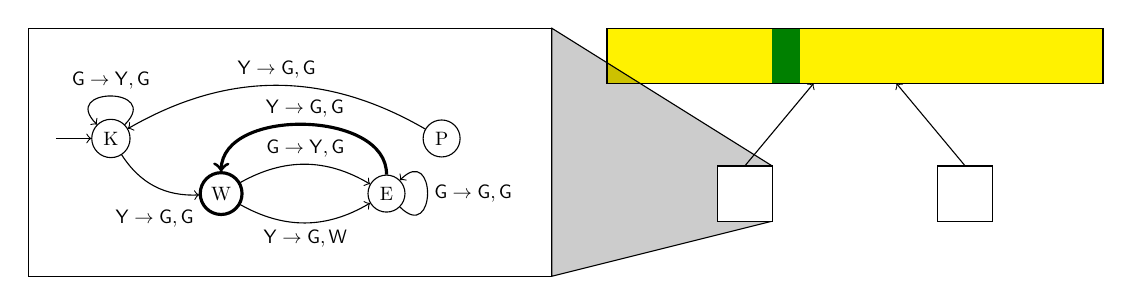
\begin{tikzpicture}[scale=0.7, every node/.style={scale=0.7}]
      % Match
      \fill[yellow] (9, 1) rectangle (18, 2);
      \fill[green!50!black] (12, 1) rectangle (12.5, 2);
      \draw (9, 1) rectangle (18, 2);
      % Machine cutout
      \draw[fill=black, fill opacity=0.2] (8, -2.5) -- (12, -1.5) -- (12, -0.5) -- (8, 2) -- (8, -2.5);
      \draw[fill=white] (11, -1.5) rectangle +(1, 1);
      \draw[->] (11.5, -0.5) -- (12.75, 1);
      \draw (15, -1.5) rectangle +(1, 1);
      \draw[->] (15.5, -0.5) -- (14.25, 1);
     
      % Internals
      \draw[fill=white] (-1.5, -2.5) rectangle (8, 2);
      \node[draw, circle] (P) at (6, 0) {P};
      \node[draw, circle, line width=0.4mm] (W) at (2, -1) {W};
      \node[draw, circle] (E) at (5, -1) {E};
      \node[draw, circle] (K) at (0, 0) {K};
      \draw[->] (-1, 0) to (K);
      \draw[->] (P) to[bend right] node[midway, above] {$\q{Y} \rightarrow \q{G}, \q{G}$} (K);
      \draw[->] (W) to[bend left] node[midway, above] {$\q{G} \rightarrow \q{Y}, \q{G}$} (E);
      \draw[->] (W) to[bend right] node[midway, below] {$\q{Y} \rightarrow \q{G}, \q{W}$} (E);
      \draw[->] (E) to[in=45, out=-45, looseness=5] node[midway, right] {$\q{G} \rightarrow \q{G}, \q{G}$} (E);
      \draw[->, line width=0.4mm] (E) to[bend right=90] node[midway, above] {$\q{Y} \rightarrow \q{G}, \q{G}$} (W);
      \draw[->] (K) to[in=135, out=45, looseness=5] node[midway, above] {$\q{G} \rightarrow \q{Y}, \q{G}$} (K);
      \draw[->] (K) to[bend right] node[midway, below=3mm] {$\q{Y} \rightarrow \q{G}, \q{G}$} (W);
     
    \end{tikzpicture}
  \end{center}

  \vspace{2em}
  \onslide<2>{
    268 million machines, two players, 72 quadrillion matches.
    
    At 100 million matches per second, we need 23 years to run all matches.
  }
\end{frame}

\begin{frame}[fragile]
  \frametitle{Detecting equivalences}

  \begin{center}
    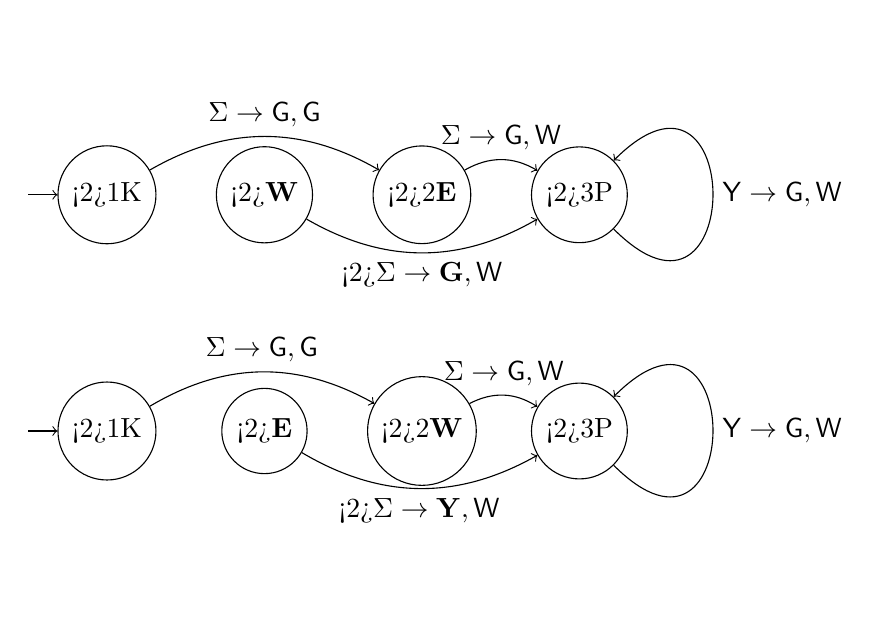
\begin{tikzpicture}
      \node[draw, circle] (P1) at (6, 0) {\alt<2>{3}{P}};
      \node[draw, circle] (W1) at (4, 0) {\alt<2>{2}{\textbf{W}}};
      \node[draw, circle] (E1) at (2, 0) {\alt<2>{}{\textbf{E}}};
      \node[draw, circle] (K1) at (0, 0) {\alt<2>{1}{K}};
      \draw[->] (-1, 0) to (K1);
      \draw[->] (P1) to[in=45, out=-45, looseness=7] node[midway, right] {$\q{Y} \rightarrow \q{G}, \q{W}$} (P1);
      \draw[->] (W1) to[bend left] node[midway, above] {$\Sigma \rightarrow \q{G}, \q{W}$} (P1);
      \draw[->] (E1) to[bend right] node[midway, below] {\alt<2>{}{$\Sigma \rightarrow \q{\mathbf{Y}}, \q{W}$}} (P1);
      \draw[->] (K1) to[bend left] node[midway, above] {$\Sigma \rightarrow \q{G}, \q{G}$} (W1);
      
      \node[draw, circle] (P2) at (6, 3) {\alt<2>{3}{P}};
      \node[draw, circle] (W2) at (2, 3) {\alt<2>{}{\textbf{W}}};
      \node[draw, circle] (E2) at (4, 3) {\alt<2>{2}{\textbf{E}}};
      \node[draw, circle] (K2) at (0, 3) {\alt<2>{1}{K}};
      \draw[->] (-1, 3) to (K2);
      \draw[->] (P2) to[in=45, out=-45, looseness=7] node[midway, right] {$\q{Y} \rightarrow \q{G}, \q{W}$} (P2);
      \draw[->] (W2) to[bend right] node[midway, below] {\alt<2>{}{$\Sigma \rightarrow \q{\mathbf{G}}, \q{W}$}} (P2);
      \draw[->] (E2) to[bend left] node[midway, above] {$\Sigma \rightarrow \q{G}, \q{W}$} (P2);
      \draw[->] (K2) to[bend left] node[midway, above] {$\Sigma \rightarrow \q{G}, \q{G}$} (E2);
    \end{tikzpicture}
  \end{center}

  \onslide<2>{
    $\frac45$ of all machines are detected duplicates;
    now 334 days at 100 million matches per second
    for 2.8 quadrillion matches.
  }
\end{frame}

\tikzset{
  match/.pic={
    % Machines
    \draw (0, 0) rectangle +(3mm, 3mm);
    \draw (1cm, 0) rectangle +(3mm, 3mm);
    \draw[->] (1.5mm, 3mm) -- (7mm, 6mm);
    \draw[->] (11.5mm, 3mm) -- (11mm, 6mm);
    % Board
    \fill[yellow] (-3mm, 6mm) rectangle +(19mm, 3mm);
    \fill[green!50!black] (3mm, 6mm) rectangle +(1mm, 3mm);
    \fill[green!50!black] (-1mm, 6mm) rectangle +(1mm, 3mm);
    \fill[green!50!black] (8mm, 6mm) rectangle +(1mm, 3mm);
    \fill[green!50!black] (13mm, 6mm) rectangle +(1mm, 3mm);
    \fill[green!50!black] (13mm, 6mm) rectangle +(1mm, 3mm);
    \draw (-3mm, 6mm) rectangle +(19mm, 3mm);
  }
}

\begin{frame}[fragile]
  \frametitle{Interpretation}

  \onslide<2->{Parallelise over multiple threads\onslide<3->{, and over multiple SIMD lanes.}}

  \begin{center}
    \begin{tikzpicture}
      \node[visible on=<2->] at (0.75, 5.7) {Core 1};
      \draw (0, 6) rectangle (8, 4.5);
      \pic at (1.8, 4.75) {match};
      \pic[visible on=<3->] at (4, 4.75) {match};
      \node[visible on=<3->] at (6.75, 5.25) {$\cdots\ (8\times)$};

      \node[visible on=<2->] at (0.75, 4.2) {Core 2};
      \draw[visible on=<2->] (0, 4.5) rectangle (8, 3);
      \pic[visible on=<2->] at (1.8, 3.25) {match};
      \pic[visible on=<3->] at (4, 3.25) {match};
      \node[visible on=<3->] at (6.75, 3.75) {$\cdots\ (8\times)$};

      \node[visible on=<2->] at (0.75, 2.7) {Core 3};
      \draw[visible on=<2->] (0, 3) rectangle (8, 1.5);
      \pic[visible on=<2->] at (1.8, 1.75) {match};
      \pic[visible on=<3->] at (4, 1.75) {match};
      \node[visible on=<3->] at (6.75, 2.25) {$\cdots\ (8\times)$};
      
      \node[visible on=<2->] at (4, 1) {$\vdots\ (24\times)$ };
    \end{tikzpicture}
  \end{center}

  \only<1>{4}\only<2>{54}\only<3>{315} million matches per second.
  \only<2>{(A $13.5\times$ improvement.)}%
  \only<3>{(A $5.8\times$ improvement on top.)}
\end{frame}

\begin{frame}
  \frametitle{Memory latency}
  \begin{columns}
    \begin{column}{0.4\textwidth}
      Where do we put results?

      \vspace{1em}

      Sharing memory hurts:
      about 76\,ns to run a match on my desktop vs.
      115\,ns median core-to-core latency on a large CPU.

      Not sharing memory hurts: results take 636\,MB.

      Duplicate work to avoid touching memory?
    \end{column}
    \begin{column}{0.6\textwidth}
      \begin{center}
        \includegraphics[height=0.8\textheight]{epyc-c2c-latency.png}

        \tiny From \url{https://github.com/nviennot/core-to-core-latency}
      \end{center}
    \end{column}
  \end{columns}
\end{frame}
\end{document}

% Local Variables:
% TeX-engine: xetex
% End:
